\documentclass{report}
\usepackage{ae,lmodern} % Polices vectorielles
\usepackage[french]{babel} % Traitement du français
\usepackage[utf8]{inputenc} % encodage d’entrée
\usepackage[T1]{fontenc} % encodage de sortie
\usepackage{moreverb} % utilisation de verbatimtab
\usepackage{verbatim} % inclure du code source
\usepackage{graphicx} % inclure des images
\usepackage[final]{pdfpages} % inclure des PDFs
\usepackage{hyperref} % inclure des adresses web
\newcommand\tab[1][5mm]{\hspace*{#1}}
\parindent=0em % Supprimer les marges en début de paragraphes.
\usepackage{parskip} % blank lines

\begin{document}
	\title{Rapport de stage}
	\author{Martin Digard}
	\date{}
	\maketitle
	\tableofcontents
	\chapter{Mois de mai}
	\section{Présentation du jeu de données}
	\textbf{groove MIDI dataset}\\
	\url{https://magenta.tensorflow.org/datasets/groove}\\\\
	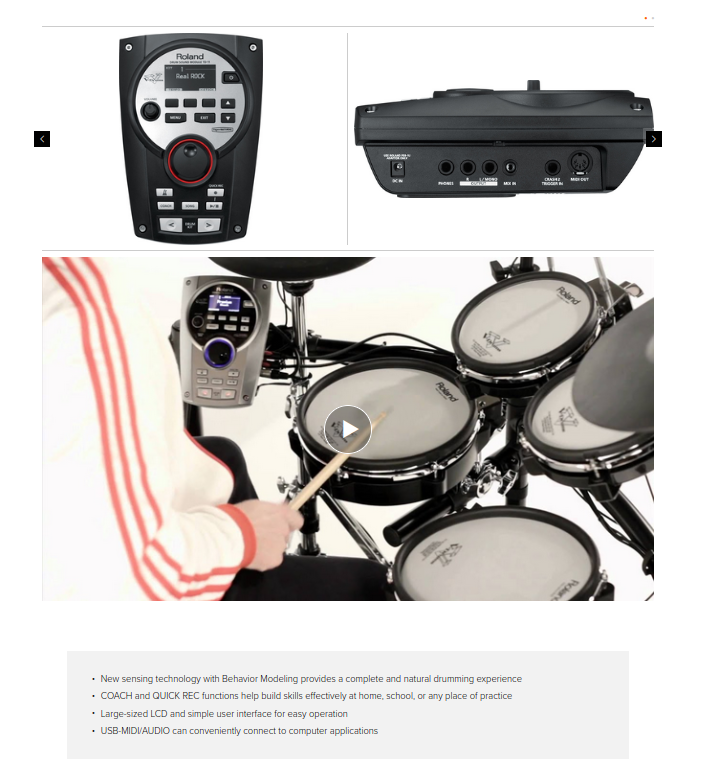
\includegraphics[height=60mm, width=60mm]{images/presentation_groove/roland_TD11.png}\\
	Des batteurs pro ont été engagés pour jouer sur un roland td-11\\\\
	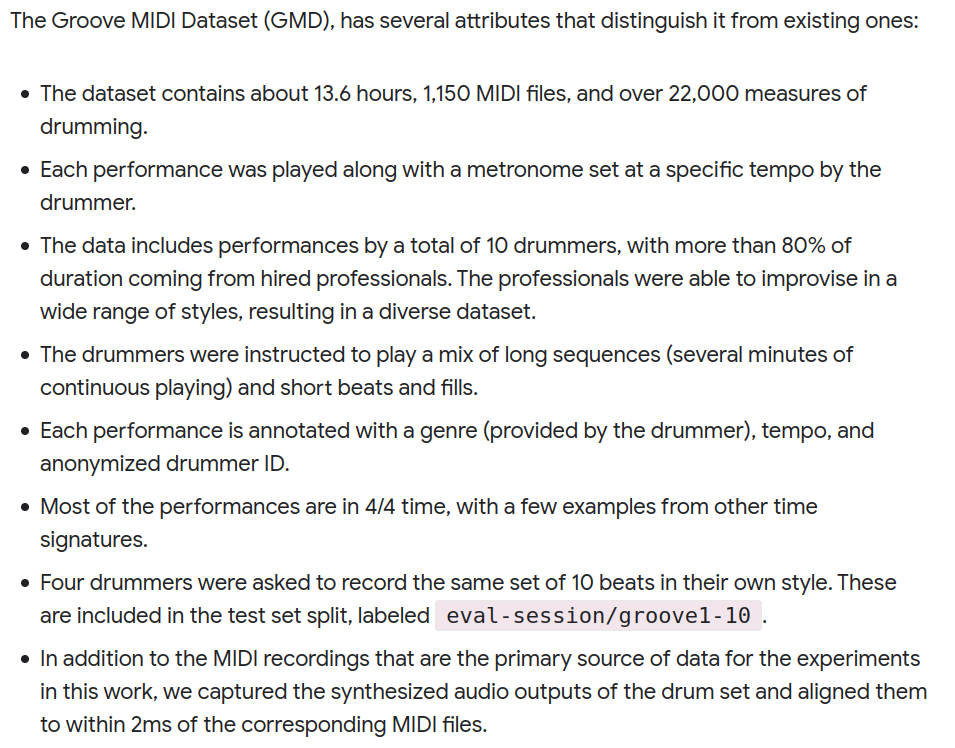
\includegraphics[height=80mm, width=110mm]{images/presentation_groove/dataset_how.png}\newpage{}
	\textbf{Les métadatas :}\\\\
	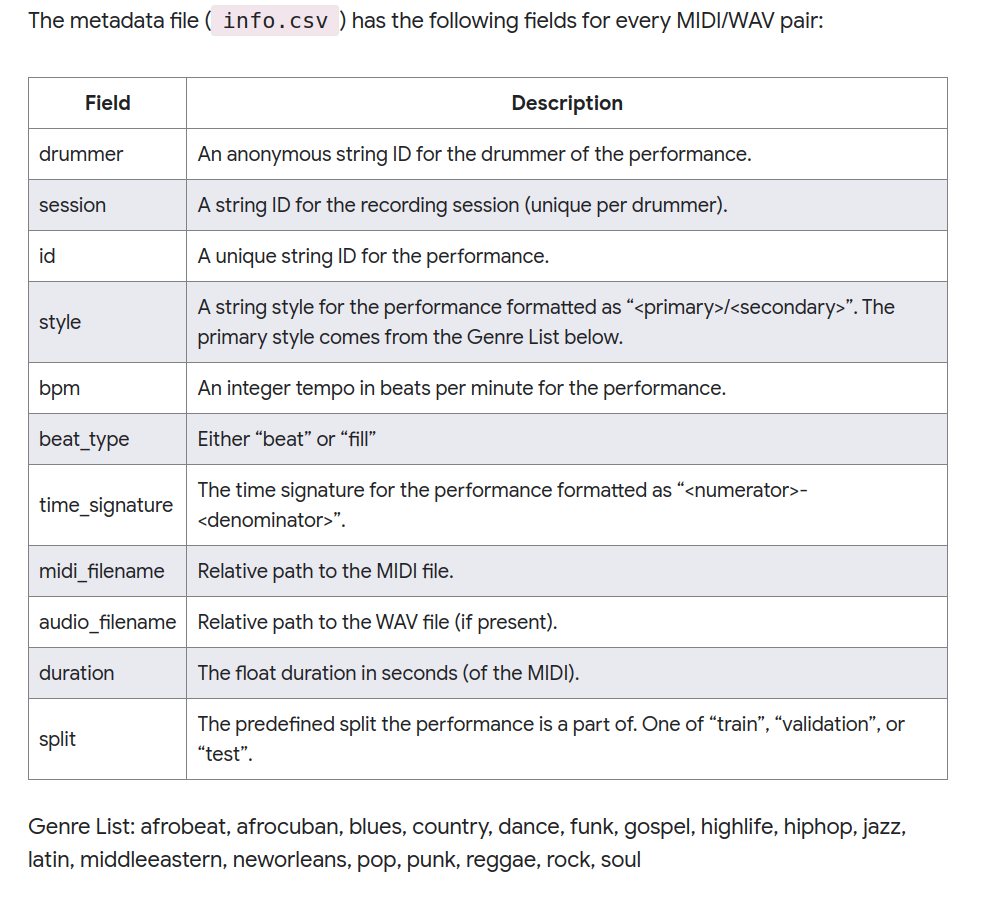
\includegraphics[height=85mm, 
	width=100mm]{images/presentation_groove/csv_metadata_struct.png}\\
	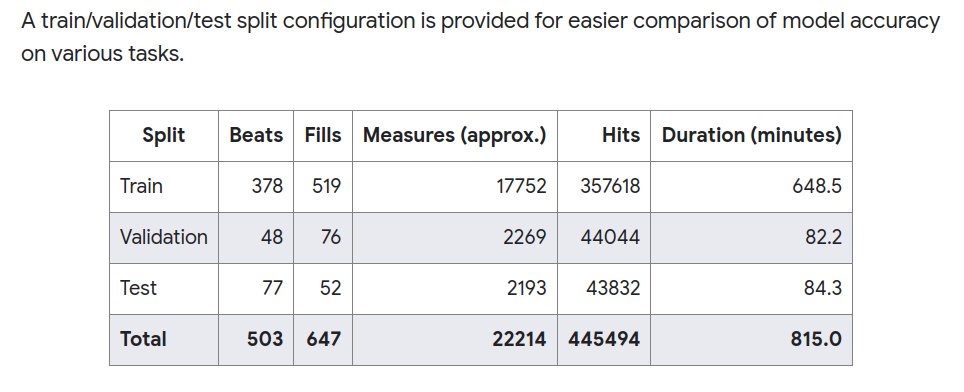
\includegraphics[height=50mm, width=120mm]{images/presentation_groove/train_validation_test.png}\\
	Détails (entre autres tensorflow avec le dataset) à :
	\url{https://magenta.tensorflow.org/datasets/groove#license}\\
	\newpage
	
	
	
	\chapter{Semaine du 7 au 11 juin}
	\section{Lundi 7 juin}
	\subsection{\textbf{Comparaisons de transcriptions}\\\textit{Manuelles vs MuseScore}}
	Les transcriptions manuelles sont faites à partir des fichiers wav et celles de MuseScore à partir des fichiers MIDI.\\
	
	\textbf{Premiers tests sur drummer\_01/session3}\\
	
	\textbf{\textit{Exemple 1 : 10\_rock-folk\_90\_beat\_4-4}}\\\\
	\textbf{manuelle}\\
	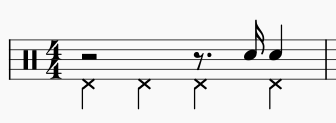
\includegraphics[height=25mm, width=70mm]{images/transcriptions_manuelles/0_prise_en_main/0_tests_drummer_01__session3/manuel_0.png} \\
	\textbf{musescore}\\
	\includegraphics[height=25mm, width=70mm]{images/transcriptions_manuelles/0_prise_en_main/0_tests_drummer_01__session3/musescore_0.png} \\
	\begin{itemize}
		\item Erreur d’indication de mesure ;
		\item Mauvaise transcription d’une noire.\\
	\end{itemize}
	La noire du 4ème temps se retrouve sur le premier temps de la mesure suivante et elle se transforme en un triolet de double croches dont seules les deux premières seraient jouées.\\\\
	\textbf{\textit{Exemple 2 : 10\_rock-folk\_90\_beat\_4-4}}\\\\
	\textbf{manuelle}\\
	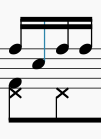
\includegraphics[height=30mm, width=25mm]{images/transcriptions_manuelles/0_prise_en_main/0_tests_drummer_01__session3/manuel_1.png} \\
	\textbf{musescore}\\
	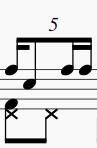
\includegraphics[height=30mm, width=25mm]{images/transcriptions_manuelles/0_prise_en_main/0_tests_drummer_01__session3/musescore_1.png} \\
	\begin{itemize}
		\item Erreur de quantification : les doubles croches ont été interprétées en quintolet;\\
	\end{itemize}
	\textbf{\textit{Exemple 3 : 2\_jazz-swing\_185\_beat\_4-4}}
	\\\\
	\textbf{manuelle}\\
	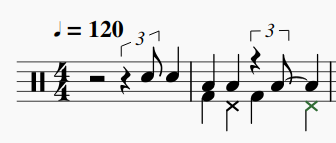
\includegraphics[height=30mm, width=65mm]{images/transcriptions_manuelles/0_prise_en_main/0_tests_drummer_01__session3/manuel_2.png} \\
	\textbf{musescore}\\
	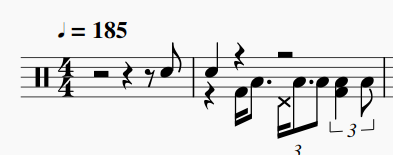
\includegraphics[height=30mm, width=65mm]{images/transcriptions_manuelles/0_prise_en_main/0_tests_drummer_01__session3/musescore_2.png} \\
	\begin{itemize}
		\item L’indication de mesure est correcte mais tout a été décalé d’un temps car la première noire sur la caisse claire est jouée sur le 4ème temps et non sur le premier temps de la deuxième mesure comme l’indique la transcription de musescore.
		\item Les toms basses des 1er et 2ème temps de la mesure musescore auraient dû être sur les temps et non décalés d’une double croche vers la droite.\\
	\end{itemize}
	\textbf{Solutions aux pb rencontrés}\\\\
	Existe-t-il un moyen de rectifier les erreurs d’indication de mesure et de décalage de temps des partitions MuseScores.\\
	\begin{itemize}
		\item Changer dans manuellement dans MuseScore l’indication de mesure\footnote{\url{https://musescore.org/fr/manuel/indications-de-mesure}} fonctionne avec la transcription du MIDI. \\\\ 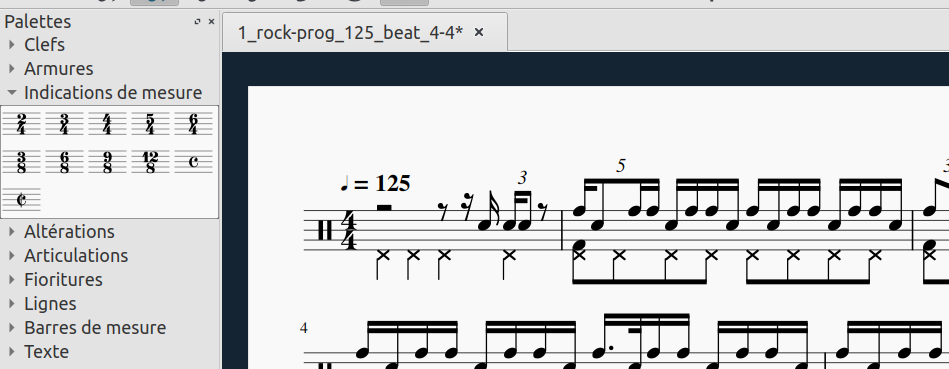
\includegraphics[height=30mm, width=65mm]{images/transcriptions_manuelles/0_prise_en_main/0_tests_drummer_01__session3/solution_0.png} \\
		\item Pour décaler tout d’un temps, on peut sélectionner les mesures en question en cliquant sur la première note de la séquence et en maj-cliquant sur la dernière, puis Ctrl-X Ctrl-V pour replacer le tout au bon endroit.\footnote{\url{https://musescore.org/fr/node/276292}}\\
	\end{itemize}
	
	\textit{À partir de la prochaine section, les indications de mesures erronées ou les décalages de temps qui ont des répercussions sur l’ensemble de la partition seront corrigés avant l’analyse.}\\\\
	\textbf{Seconds tests sur drummer\_01/session1}\\\\
	\textbf{\textit{Exemple 1 : 1\_funk\_80\_beat\_4-4}}
	\textbf{manuelle}\\
	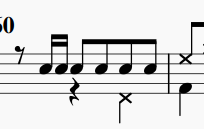
\includegraphics[height=25mm, width=40mm]{images/transcriptions_manuelles/0_prise_en_main/1_drummer_01__session1/Manuelle_0.png} \\
	\textbf{musescore}\\
	\includegraphics[height=25mm, width=40mm]{images/transcriptions_manuelles/0_prise_en_main/1_drummer_01__session1/musescore_0.png} \\
	\begin{itemize}
		\item On dirait que lorsque certaines notes sont proches, elles se resserrent et suppriment celles qui aurait dû être sur le temps.\\
	\end{itemize}
	\textbf{\textit{Exemple 2 : 1\_funk\_80\_beat\_4-4}}
	1\_funk\_80\_beat\_4-4\\\\
	\textbf{manuelle}\\
	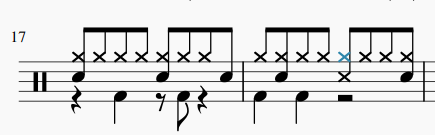
\includegraphics[height=25mm, width=70mm]{images/transcriptions_manuelles/0_prise_en_main/1_drummer_01__session1/Manuelle_1.png} \\
	\textbf{musescore}\\
	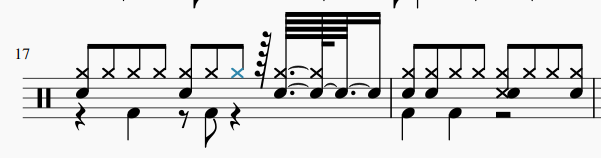
\includegraphics[height=25mm, width=70mm]{images/transcriptions_manuelles/0_prise_en_main/1_drummer_01__session1/MuseScore_1.png} \\
	\begin{itemize}
		\item La caisse claire de la 2ème croche du 4ème temps de la 1ère mesure se transforme en une combinaison de quadruple/quintuple/double croches liées qui commence par un soupir et finit en débordant sur le premier temps de la mesure suivante. 
	\end{itemize}
\newpage
	\section{Mardi 8 juin}
	\subsection{Écriture de partitions}
	Les partitions pour la transcription manuelle seront écrites avec LilyPond.\\\\
	Voici un exemple de code :
	\begin{verbatimtab}
	\version "2.22.1"
	\language français
	{
		do' re' mi' fa' sol' la' si' do'' re'' mi'' fa'' sol'' la'' si'' do'''
	}
	\relative {
		do' re mi fa sol la si do re mi fa sol la si do
	}
	\relative {
		do'4. do4. do4
		mi2 re
		do16 do do do do do8 do16 do do do do do do8 do16
		mi8 mi mi mi re re re re
	}
	\end{verbatimtab}
	Avec la commande :\begin{verbatim}$ lilypond fichier.ly\end{verbatim}:
	On obtient le pdf suivant :\\
	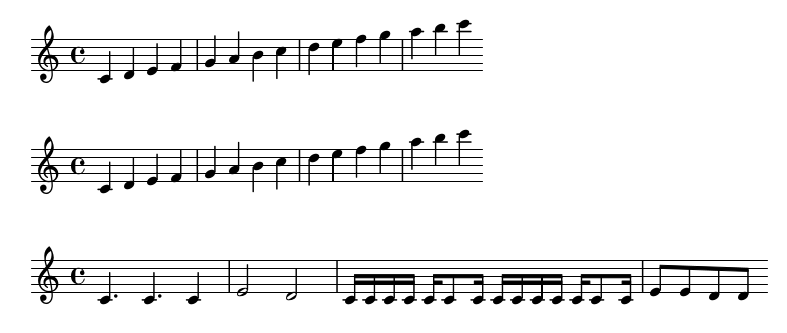
\includegraphics[height=50mm, width=110mm]{images/lilypond_0.png}\\\\
	\textbf{Bases :}\\
	\url{http://lilypond.org/doc/v2.22/Documentation/learning/simple-notation}\\
	
	\textbf{Percussions et batterie :}\\
	\url{http://lilypond.org/doc/v2.22/Documentation/notation/common-notation-for-percussion}
	\newpage
	\section{Mercredi 9 juin}
	\subsection{Recherche de flas dans groove}
	Les noms des fichiers ont été normalisés avec le script suivant :
	\begin{verbatimtab}
	$ cat ordered_files.sh 
	echo
	for drummer in `ls | egrep drummer_`
	do
		echo $drummer
		echo
		for session in `ls $drummer | egrep ^session`
		do
			echo $session
			echo
			cd $drummer/$session
			rename 's/^([0-9])_/00$1_/' *.* 
			rename 's/^([0-9]{2})_/0$1_/' *.* 
			ls -1 *.*
			echo
			cd ../..
		done
		echo "**********"
		echo
		echo
	done
	echo
	\end{verbatimtab}
	L’objectif est de les avoir dans le même ordre aussi bien dans le terminal que dans
	l’interface graphique. C’est plus facile pour la récupération des noms lors d’une écoute.
	\begin{verbatim}
	« …
	007_jazz-funk_116_fill_4-4.wav
	008_jazz-funk_116_fill_4-4.mid
	008_jazz-funk_116_fill_4-4.wav
	009_jazz-funk_116_fill_4-4.mid
	009_jazz-funk_116_fill_4-4.wav
	010_jazz-funk_116_fill_4-4.mid
	010_jazz-funk_116_fill_4-4.wav
	011_jazz-funk_116_fill_4-4.mid
	011_jazz-funk_116_fill_4-4.wav
	… »
	\end{verbatim}
	\newpage
	\begin{verbatim}
	\$ cat fichiers_contenant_des_flas 
	
	Dans drummer_01/session1 :
	
	003_funk_80_beat_4-4.wav
	005_jazz-funk_116_beat_4-4
	012_jazz-funk_116_fill_4-4
	016_jazz-funk_116_fill_4-4
	019_jazz-funk_116_fill_4-4
	020_jazz-funk_116_fill_4-4
	024_jazz-funk_116_fill_4-4
	038_latin-samba_116_beat_4-4 (00:55)
	039_latin-samba_116_fill_4-4
	040_latin-samba_116_fill_4-4
	043_latin-samba_116_fill_4-4
	044_latin-samba_116_fill_4-4
	045_latin-samba_116_fill_4-4
	046_latin-samba_116_fill_4-4
	047_jazz_102_beat_4-4
	048_jazz_93_beat_4-4
	049_jazz_125_beat_4-4 (cc-tom)
	051_rock-shuffle_125_beat_4-4
	054_jazz_125_fill_4-4 (cc-tom)
	055_jazz_125_fill_4-4 (cc-tom)
	073_jazz_125_fill_4-4
	077_jazz-mediumfast_180_beat_4-4 (cc-tom, vers le milieu)
	082_neworleans-funk_84_beat_4-4 (vers le milieu)
	085_neworleans-funk_84_fill_4-4 (cc-tom)
	093_neworleans-funk_84_fill_4-4
	094_neworleans-funk_84_fill_4-4
	095_neworleans-funk_84_fill_4-4
	096_neworleans-funk_84_fill_4-4
	099_neworleans-funk_84_fill_4-4
	\end{verbatim}
	Questions :
	
	- Les flas caisse-claire/tom sont-ils intéressants ?
	\newpage
	\section{Jeudi 10 juin}
	\subsection{Recherche de flas dans groove (suite)}
	\begin{verbatim}
		101_dance-disco_120_beat_4-4 (00:55)
	102_funk_95_beat_4-4
	107_funk_95_fill_4-4
	108_funk_95_fill_4-4
	111_funk_95_fill_4-4
	112_funk_95_fill_4-4
	113_funk_95_fill_4-4
	114_funk_95_fill_4-4
	115_funk_95_fill_4-4
	116_funk_95_fill_4-4
	118_funk_95_fill_4-4
	119_funk_95_fill_4-4
	120_funk_95_fill_4-4
	123_funk_95_fill_4-4
	124_funk_95_fill_4-4
	\end{verbatim}
	\subsection{Cours de batterie}
	2 élèves le jeudi soir.
	\newpage
	\section{Vendredi 11 juin}
	\subsection{Rassemblement d’ouvrages d’ouvrages de référence sur la notation}
	\textbf{Méthodes Agostini :}
	\begin{itemize}
		\item solfèges rythmiques n° 1, 2, 3, 4 ;
		\item Méthodes de batterie n° 1, 2, 3, 4 ;
		\item Rythmiques binaires n° 1, 2 (J.-F. Juskowiak).\\
	\end{itemize}
	\textbf{Méthodes américaines :}\\
	Une dizaine de méthodes américaines ont été rassemblées car leur système de notation diffère légèrement de celui des méthodes agostini.\\
	
	\textbf{Autres ouvrages sur la batterie :}
	\begin{itemize}
		\item Une histoire de la batterie de jazz, Georges Paczynski.
		\item Rythme et geste, Georges Paczynski.\\
	\end{itemize}
	\textbf{Autres références sur la notation musicale :}
\begin{itemize}
	\item A. Danhauser, édition revue et augmentée
	Elle contient notamment des informations en plus l’écriture des métriques ;
	\item Behind Bars, the definitive guide to music notation, Elaine Gould.\\
\end{itemize}
\subsection{Mémoire de recherche}
Création d’un template en LateX pour le mémoire de recherche.\\\\
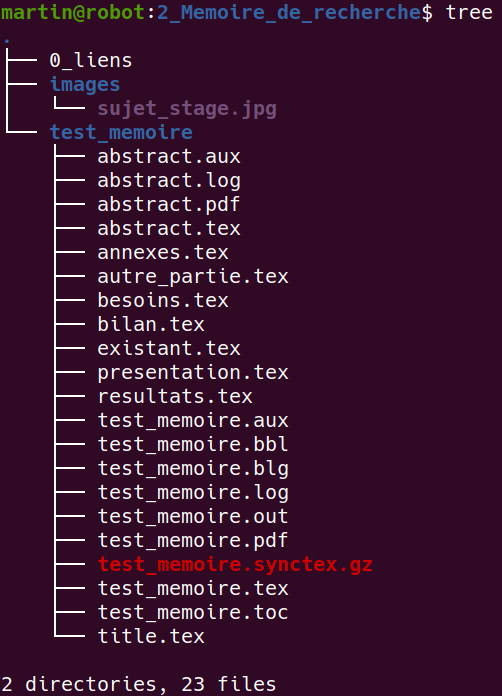
\includegraphics[height=80mm, width=60mm]{images/test_memoire_0.png}\\

\newpage
	\chapter{Semaine du 14 au 18 juin}
	\section{Lundi 14 juin}
	\subsection{Sur la question des flas}
	Des exemples de notation flas tom/caisse-claire existent dans des partitions récentes (rythmique binaire J.-F. Juskowiak).\\
	$\Rightarrow$ Ils faudra donc les prendre en compte dans les comparaisons de transcriptions.
	\subsection{Prise en main d’un clavier ergonomique}
	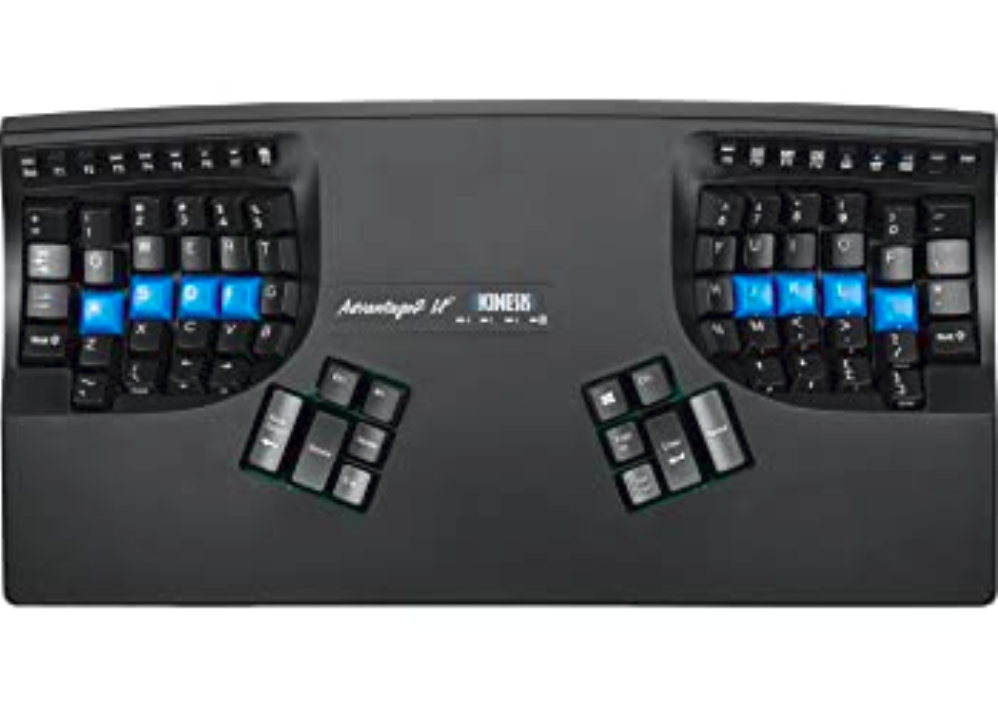
\includegraphics[height=50mm, width=70mm]{images/clavier_ergo_0.png}\\
	Désolé, ça prend du temps mais c’est important.
	\newpage
	\section{Mardi 15 juin}
	\subsection{Description de la notation de la batterie}
	Document page suivante.\newpage
	—————————————————————————————————————————————————————————————————————————————————————\\
\begin{center}
	\textbf{\LARGE{Description de la notation de la batterie}}
\end{center}
\section*{1. Petit État de l’art}
\subsection*{Notation américaine}
Dans la notation américaine, les cymbales sont plus basses dans la portée et la grosse caisse, le tom basse et la caisse-claire sont montés d’un ton ou d’un demi ton dans la portée.
\subsection*{Notation Agostini}
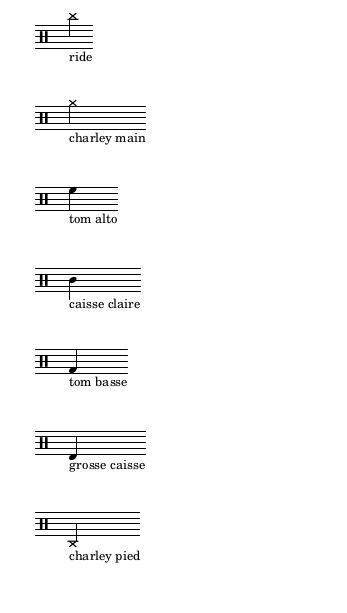
\includegraphics[height=150mm, width=90mm]{images/description_notation_0.png}\\
Il faudra ajouter :
\begin{itemize}
	\item le cross-cut
	\item les ghost-notes
\end{itemize}
\subsection*{Notation des flas}
\textit{À faire :}
\begin{itemize}
	\item Trouver des flas dans les méthodes américaines\\
\end{itemize}
On considère comme un fla deux frappes très proches non-synchrones et qui ne sont pas quantifiées. La première de ces deux notes est une appogiature. En batterie, elle peut-être jouée piano ou avec la même force que la suivante.
L’écriture des flas ressemble à celle des appogiatures même si cette dernière place la note ornementale à un degré (ton ou demi-ton) au-dessus ou au-dessous de la note principale.\footnote{Théorie de la musique, A. Danhauser}
\section*{2. Définition des symboles et des hauteurs}
\subsection*{Proposition de définition d’un standard de départ}
Pour la transcriptions, nous proposons de choisir la base Agostini. La caisse claire centrale sur la portée est aussi centrale sur la batterie est elle est un élément qui conditionne la position des jambes (écart entre les pédales, etc.) ainsi que l’organisation des éléments en hauteur (toms, cymbales, etc.).
On pensera en terme de symétrie la répartition des éléments par rapport au point central que constitue la caisse claire.\\
Cette symétrie s’opère en trois dimensions :
\begin{itemize}
	\item Les hauteurs en terme de fréquences ;
	\item La hauteur physique des éléments :\\
	Du bas vers le haut : pédales, toms et caisse, cymbales
	\item L’ergonomie, qui hiérarchise l’importance des éléments sur la portée (caisse claire au centre, hh-pied et ride sont aux deux extrémités).
\end{itemize}
\section*{3. Direction des hampes et des ligatures}
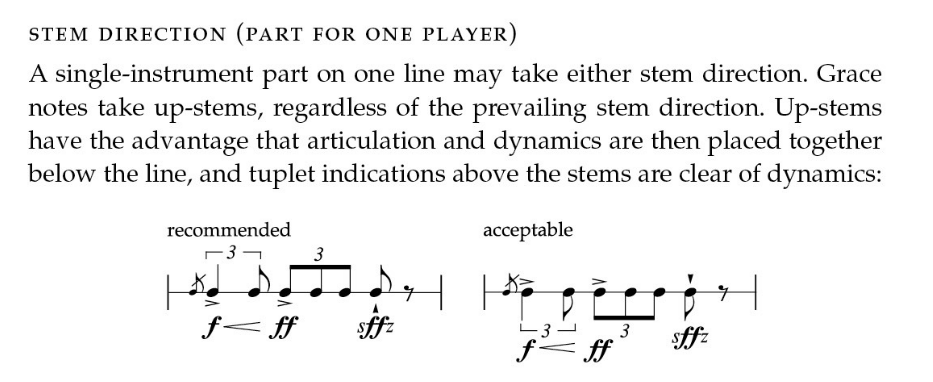
\includegraphics[height=60mm, width=120mm]{images/hampes_0.png} \\\textit{Source : Behind Bars, Elaine Gould}\\\\
Le principe ci-dessus semble être respecté dans les rythmiques binaires de Juskowiac mais pas dans les Méthodes agostini\\

\textbf{Quelques idées :}\\
\begin{itemize}
	\item \textbf{\textit{Les systèmes :}}\\
	$\Rightarrow$ Un système est la combinaison d’un ou plusieurs éléments qui jouent un rythme en boucle (système) et d’un autre élément qui joue un \textit{texte} rythmique variable mais respectant les règles propre au système (texte).\\
	En cas de système, les ligatures forment deux voies :
	\begin{itemize}
		\item Le texte ;
		\item Le système.
	\end{itemize}
	\textit{Mettre des exemples de différents systèmes.}
	\item \textbf{\textit{Les moulins :}}\\
	Lorsqu’il y a plus d’une voie, ils sont prioritaires pour les ligatures.\\
	\textit{Mettre des exemples.}\\
\end{itemize}
—————————————————————————————————————————————————————————————————————————————————————\\\\
	Retour au document principal page suivante.\newpage
La définition des symboles a été faite avec lilypond avec le script suivant :
\begin{verbatimtab}
	$ cat description_notation_0.ly 
	
	\version "2.22.1"
	\language français
	
	{
		% Toutes les hauteurs sont en ut
		\clef percussion
		
		% Ne pas appeler la fonction qui dessine les symboles
		\override Staff.TimeSignature.stencil = ##f 
		
		% Changer la tête de note
		\override NoteHead.style = #'cross
		
		% Hauteur de la note + commentaire
		do''-"ride"
	}

	{
		\clef percussion
		\override Staff.TimeSignature.stencil = ##f
		\override NoteHead.style = #'cross
		la'-"charley main"
	}

	{
		\clef percussion
		\override Staff.TimeSignature.stencil = ##f
		fa'-"tom alto"
	}
	
	{
		\clef percussion
		\override Staff.TimeSignature.stencil = ##f
		do'-"caisse claire"
	}

	{
		\clef percussion
		\override Staff.TimeSignature.stencil = ##f
		sol-"tom basse"
	}

	{
		\clef percussion
		\override Staff.TimeSignature.stencil = ##f
		mi-"grosse caisse"
	}

	{
		\clef percussion
		\override Staff.TimeSignature.stencil = ##f
		\override NoteHead.style = #'cross
		do-"charley pied"
	}
\end{verbatimtab}
	\newpage
	\section{Mercredi 16 juin}
	\subsubsection{Clavier ergonomique et bépo}
	Dernier réglages, keybindings et dactylotest (bépo)
	\section{Jeudi 17 juin}
	\begin{itemize}
		\item Installation de cmake-3.20.4 ;
		\item Ajout de quelques idées pour la notation des ligatures\\\textit{(Voir 3.2.1 Description de la notation de la batterie)} ;
		\item Installation d’un environnement pour le C++.
	\end{itemize}
\subsection{Comparaisons de transcriptions}
\textit{À faire :}
\begin{itemize}
	\item Flas\\\textit{À partir des fichiers déjà collectés} ;
	\item Autres…\\
\end{itemize}
Début du document sur la page suivante.\newpage
—————————————————————————————————————————————————————————————————————————————————————\\
\begin{center}
	\textbf{\LARGE{Comparaisons de transcriptions}}
\end{center}
\section*{1. Transcription des flas}
De gauche à droite : transcription musescore, transcription manuelle.\\
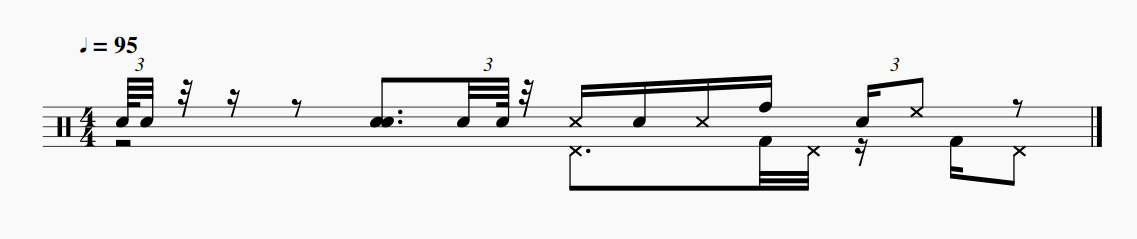
\includegraphics[height=20mm, width=80mm]{images/transcriptions_manuelles/1_transcriptions_flas/124_funk_95_fill_4-4_0.png}
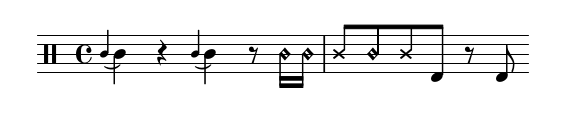
\includegraphics[height=20mm, width=80mm]{images/transcriptions_manuelles/1_transcriptions_flas/124_funk_95_fill_4-4_1.png}\\
Il manque des charley, je dois trouver comment faire des accords avec des têtes de notes différentes.\\\\
—————————————————————————————————————————————————————————————————————————————————————\\\\

Retour au document principal sur la page suivante.\newpage
Début du document sur la page suivante.\newpage
—————————————————————————————————————————————————————————————————————————————————————\\
\begin{center}
	\textbf{\LARGE{Lilypond}}
\end{center}
Endroit pour les fichiers de la drum :\\
/home/martin/lilypond/usr/share/lilypond/current/ly/drumpitch-init.ly\\\\
—————————————————————————————————————————————————————————————————————————————————————\\\\

Retour au document principal sur la page suivante.\newpage
\end{document}
